\chapter[Uniform Field TE01U Cavity at Q-band Frequencies]{Uniform Field Re-Entrant TE$_{01\text{U}}$ Cavity at Q-band Frequencies.\blfootnote{A significant portion of this chapter is from J.~W.~Sidabras, E.~J.~Reijerse, W.~Lubitz, Appl. Magn. Reson. 48~(11) (2017) 1301--1314.}}

Since the introduction of uniform field resonators by Mett \textit{et al.}, uniform field resonator geometries have been extended from cavity-based \cite{mett2001axially,anderson2002,mett2002recav,hyde2004cavity} to loop-gap based resonators. \cite{UFLGR} Recently, a uniform field resonator at X-band (9.5~GHz) with a dielectric insert was introduced by Mett \textit{et al.} in order to increase EPR sensitivity without creating an overly large cavity. \cite{HydeUFDR2017} At Q-band (35~GHz), we introduced re-entrant protrusions into a cavity resonator in order to increase the resonator efficiency for pulse experiments (Chapter~3). \cite{SidabrasReEnt2017} The re-entrant protrusions bridge the geometrical gap between cavity and loop-gap resonators. In 2017, Sidabras \textit{et al.} fabricated a rectangular TE$_{\text{U}02}$ with light-access slots and a loop-gap resonator with magnetic field enhancement end-sections extending the implementation of uniform field resonators to W-band (94~Ghz). \cite{UFLGR2017} These advances in resonator design have been recently reviewed. \cite{HydeUFRev2019} In this section, the underlying understanding behind uniform field resonators will be described.

Uniform field resonators have a number of advantages for both continuous-wave and pulse EPR experiments. In continuous-wave EPR at low power, a uniform field resonator with the same active sample volume as traditional cavity will increase the EPR signal by the ratio of the square of the magnetic field between the cavities. However, in a traditional cavity at an incident power high enough to cause saturation a distribution of the magnetic field exists along the sample. By increasing the uniformity of the magnetic field all spins along the sample length are saturated at the same value. This has direct implications in the quality of data obtained from a sampled under saturation conditions. For example, in saturation transfer experiments where the out-of-phase component of the phase-sensitive detector is used as an indicator of molecular motion as the sample is driven under saturation conditions. \cite{SaturationTransfer2005} 

Uniform field resonators used in pulse experiments will not only increase the the EPR signal, but time-dependent effects that may lead to complex backgrounds can be reduced. The effects of non-uniform magnetic field excitation are relatively unknown as the number of pulses increase in more sophisticated sequences. In general, uniform field resonators increase the quality of pulse data and reduce artifacts.

\subsection*{Design and implementation of Uniform Field Resonators.}
We start by introducing the cylindrical waveguide where the two-dimensional wave equation describes the transverse electric (TE) modes that propagate along the $\pm z$-direction, such that
\begin{equation}
    (\bigtriangledown_t^2 + \beta_{mn}^2) \mathbf{H}_z = 0,
\end{equation}
where the magnetic field $\mathbf{H}_z$ mode is set by the scalar solution of the transverse components in the $\rho$ and $\phi$ coordinates for a time-varying electromagnetic field $e^{-i \omega t}$. Illustrated in Fig.~\ref{fig:UFwaveguide} is a cylindrical waveguide with a radius of $a$, and the propagation constant can be expressed as a function of the roots of the derivative of the Bessel function of the first kind, such that
\begin{equation}
    \beta_{mn}^2 = \beta_0^2 - \beta_\rho^2 = \beta_0^2 - \bigg(\frac{J_{mn}'}{a}\bigg)^2,
\end{equation}
where $J_{mn}'$ is the $n$-th zero in the first-derivative of the Bessel function $J_m(x)$ and $\beta_0$ is the free-space propagation constant $\omega\sqrt{\epsilon_r \mu_r}$. When $\beta_{mn}$ is set to zero and solved for the frequency the ``cut-off'' condition can be calculated, such that
\begin{equation}
    \omega_c = \frac{1}{\sqrt{\epsilon_r \mu_r}}\frac{J_{mn}'}{a} \qquad [\text{Hz}].
\end{equation}
For the TE$_{01}$ mode, the $J_{01}'$ is approximately 3.832. For simplicity, we assume there is no perturbation from the coupling iris. When the operating frequency $f$ is greater than $f_c$ and the waveguide is infinitely long, the electromagnetic wave will propagate,
\begin{equation}
    \mathbf{H}_z = e^{\pm i\beta_{01}z},\label{propH}
\end{equation}
in the $\pm z$-direction and the wavelength in the waveguide $\lambda_g$ will be determined by 
\begin{equation}
    \lambda_g = \frac{2\pi}{\beta_0 \sqrt{1-(f_c/f)^2}} \qquad [\text{m}].\label{wavelength}
\end{equation}
This is illustrated in Fig.~\ref{fig:UFwaveguide}A as the magnitude of the magnetic field and plotted on axis to the right of the geometry. As the operating frequency increases the propagating wavelength approaches the free-space wavelength. \cite{harrington1961time} 

\begin{figure}[ht]
 \centering
 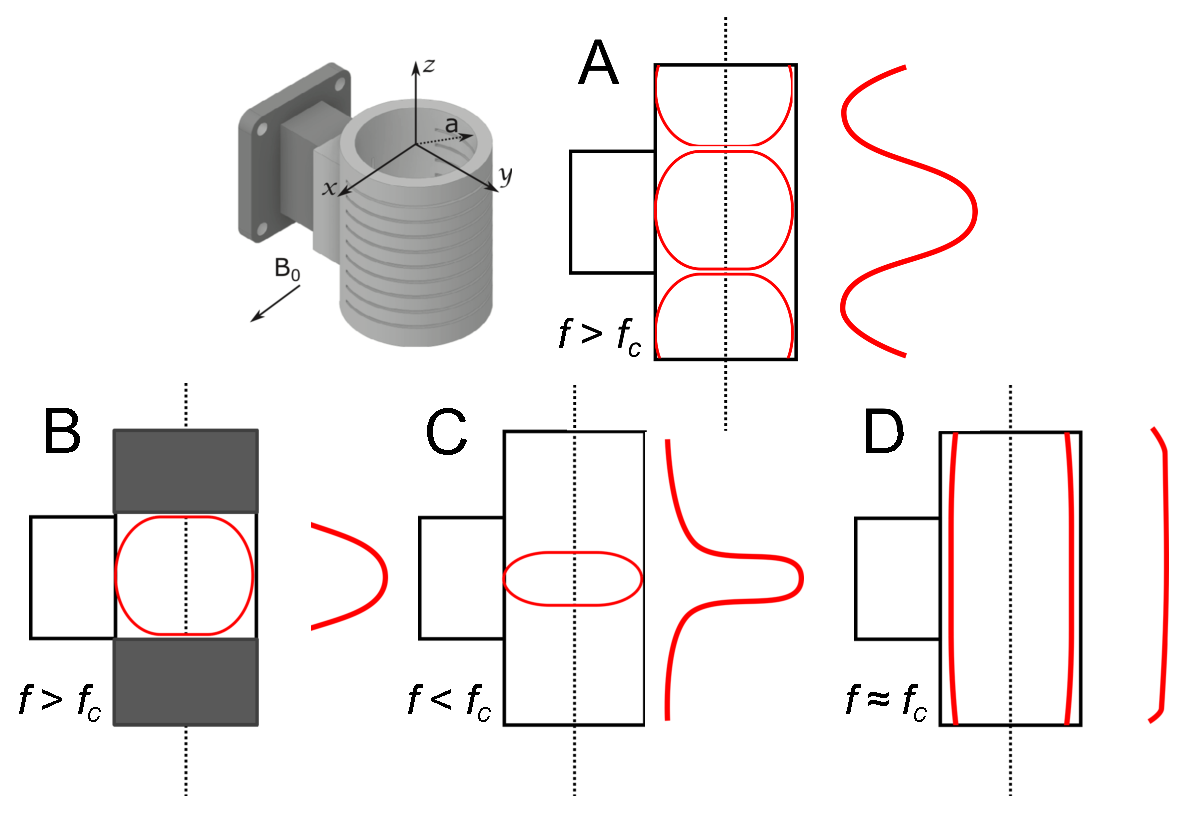
\includegraphics[width=0.9\textwidth]{Kapitel/Ch2-Images/Ch2-UniformFieldWaveguide.eps}
 \caption[Waveguide modes relative to the cut-off frequency]{Waveguide modes relative to the cut-off frequency. A cylindrical waveguide with a radius of $a$ is coupled to a rectangular waveguide, shown in the inset. The static magnetic field $B_0$ is indicated in the $x$-direction. A) When the operating frequency $f$ is greater than the cut-off frequency $f_c$ propagation occurs in the $\pm z$-direction. B) When conducting end caps are added, a cavity is created. C) If the operating frequency is less than the cut-off frequency ($f < f_c$) an evanescent mode is formed. D) When the operating frequency approaches the cut-off frequency ($f \approx f_c$) the wavelength becomes infinite, resulting in a uniform field. }
 \label{fig:UFwaveguide}
\end{figure}

By adding end caps to a waveguide a boundary condition is imposed on the TE$_{01}$ propagating mode which forces tangential electric field to zero resulting in a cosine dependence of the magnetic field within the cavity, illustrated in Fig.~\ref{fig:UFwaveguide}B. With proper dimensions, this results in a TE$_{011}$ cavity. In EPR, a sample is placed in the maximum magnetic field where the operating frequency (X-band, Q-band, etc) is the frequency of the cavity. 

In the cylindrical waveguide, if the operating frequency $f$ is below the cut-off frequency $f_c$, the propagation constant becomes imaginary. The wave no longer propagates and, instead, $\mathbf{H}_z$ of Eqn.~\ref{propH} becomes evanescent with a reduction that is proportional to the propagation constant. 

Of interest is when the operating frequency approaches the cut-off frequency ($f \approx f_c$) the wavelength approaches infinity as described by Eqn.~\ref{wavelength}. At this condition is where uniform field resonators operate. Three characteristics describe the electromagnetic wave in the waveguide at cut-off. First, the wavelength is infinite and, therefore, the field is strictly uniform in the $\pm z$-direction for an infinitely-long waveguide. Second, the propagation constant is zero indicating no dispersion or phase velocity. This implies that a resonator with a uniform field active-region longer than a wavelength will not have a propagation time and the whole geometry will act as a single-mode cavity.  Finally, strictly uniform field in the waveguide occurs only when the operating frequency is at the cut-off frequency ($f=f_c$). Any deviation from this equality will result in either a bowed ($f>f_c$) or a concave ($f<f_c$) field profile.

The characteristic impedance of a cylindrical waveguide TE$_{01}$ is defined by 
\begin{equation}
    Z_{01} = \frac{\beta_0 \sqrt{\mu_r/ \epsilon_r}}{\beta_{01}} =\frac{\beta_0 \sqrt{\mu_r/ \epsilon_r}}{\beta_0 \sqrt{1-(f_c/f)^2}} \qquad [\Omega]
\end{equation}
and, therefore, when ($f=f_c$) the impedance approaches infinity. If we choose to create a finite-length waveguide, the reflections from the open end section would cause the formation of other modes, degrading the uniform field. If we choose to place end sections, a TE$_{01n}$ mode will form at a frequency dictated by the characteristic equation
\begin{equation}
    \omega_{01n} = \frac{1}{\sqrt{\mu_r \epsilon_r}}\sqrt{\bigg(\frac{2 \pi n}{h}\bigg)^2+\bigg(\frac{J_{01}'}{a}\bigg)^2} \qquad [\text{Hz}],
\end{equation}
where $h$ is the height of the resonator and $n$ is the number of half wavelengths that are formed.

In order for the maintain the properties of the uniform field and to to satisfy Maxwell's equations for a finite-length waveguide, the end sections must maintain a infinite characteristic impedance. An infinite characteristic impedance is likened to an ``open'' circuit and with a TE$_{01}$ mode the ``open'' circuit is a perfect-magnetic boundary condition that must be matched to the central section. 

Three matching methods were shown to produce this effect: i) over-sized end-sections above cut-off, ii) re-entrant metallic structures that adding capacitance to the end-section, and iii) dielectric end-sections of length $\lambda/4$ placed at each shorted end. All end-section types present an rf open impedance boundary condition to the central cut-off section. These methods are illustrated in Fig.~\ref{fig:UFmethods}.

\begin{figure}[htp]
 \centering
 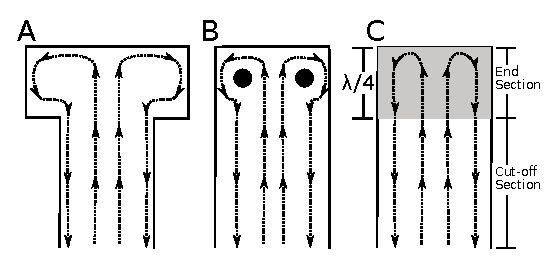
\includegraphics[width=0.7\textwidth]{Kapitel/Ch2-Images/02-UFIllustration.eps}
 \caption[Methods for creating uniform fields in cavities.]{Illustrations of three methods for creating uniform fields in cavities. Region-of-interest at cut-off is matched to A) an  over-sized section, B) a re-entrant end-section with capacitive posts (black circles), C) a dielectric section of length $\lambda/4$ placed at a shorted end. Magnetic fields vectors are illustrated with dotted lines.}
 \label{fig:UFmethods}
\end{figure}

Each method creates an end-section that transfers the characteristic impedance of a ``short'' to an ``open''. One drawback of the uniform field resonator is the frequency dependence of the whole structure. While designing a uniform field resonator, all perturbations must be accounted for, such as, the sample, sample holder, end-section dielectrics, iris, and conductivity of the cavity walls. All factors modify the cut-off frequency. Typically uniform field resonators are designed for a range of samples where the non-uniformity is quantified within a dielectric constant range. 



With the introduction of uniform field resonators for Electron Paramagnetic Resonance (EPR) spectroscopy, a cavity can be designed to have a microwave magnetic field (B$_1$) strictly uniform over a region-of-interest of any length. \cite{mett2001axially, anderson2002, mett2002recav, hyde2004cavity} However, as one increases the length of the region-of-interest, the resonator efficiency is lowered due to the reduction of stored energy within the cavity volume. By extending the uniform field concept to loop-gap resonators,\cite{UFLGR} it became possible to design resonators with both high efficiency and uniform field distributions. \cite{UFLGR2017}  

Yet, as one designs higher frequency loop-gap resonators (LGR), the sample loop diameter must be significantly reduced to lower inductance and/or the number of gaps must be increased to lower capacitance. \cite{Sidabras2007, MainaliLGR, UFLGR2017} The sample loop diameter imposes a limit on the capillary size and sample volume, potentially limiting concentration sensitivity. This limit is not present in typical cavities, such as the cylindrical TE$_{011}$ with a capillary sample, where a broad sample volume optimum exists. \cite{Nesmelov2004}

\begin{figure}[htp]\centering
 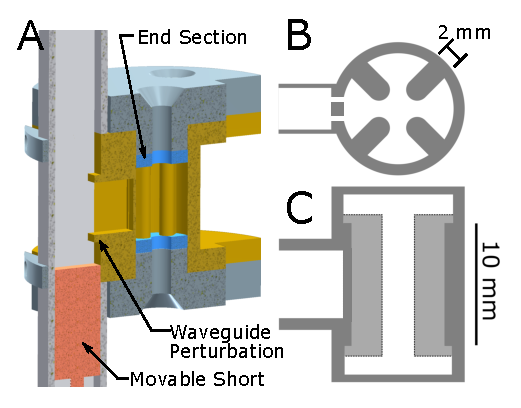
\includegraphics{Kapitel/Ch2-Images/01-TE01UGeometry.eps}
 \caption[Resonator Assembly CAD Drawing.]{A) Half-structure resonator assembly CAD drawing showing the brass resonator (gold), brass end plates (grey), Rexolite end-sections (blue), and copper waveguide (light grey). The waveguide H-type T-junction coupler with inductive obstacles and brass movable short is also illustrated. The re-entrant geometry is further detailed in B) the top view, showing the re-entrant fins and dual-slot iris, and C) the side view, showing the 10~mm uniform field region-of-interest.}
 \label{Ch2-fig:GEO}
\end{figure}

In this work we introduce a uniform field (UF) re-entrant cylindrical \cylTE{} cavity for Q-band (34~GHz) pulse EPR spectroscopy, illustrated in Fig.~\ref{Ch2-fig:GEO}. Re-entrant geometries are defined as waveguide structures where perturbations are placed in regions of large electric field in order to lower the cut-off frequency of the waveguide and increase the stored energy of the cavity. \cite{ramo1984fields, MITRadWaveguide} In a cylindrical waveguide, for a fixed cut-off frequency, the diameter of the waveguide is decreased as the re-entrant perturbations are extended into the electric field. If one was to make a re-entrant cavity by placing a shorted top/bottom on the waveguide and the resonant frequency is held constant, the stored energy of the cavity would increase as the re-entrant perturbations are increased. When sufficiently close, the re-entrant perturbations behave like plate capacitors. In fact, a LGR can be considered a highly re-entrant waveguide operating at cutoff. It is the geometric space between cavities and LGRs that the re-entrant geometry explores. 

In the present design, four 2~mm re-entrant fins are extended into a UF cylindrical \cylTE{} cavity, shown in Fig.~\ref{Ch2-fig:GEO}B, and the UF region-of-interest is elongated to 10~mm, shown in Fig.~\ref{Ch2-fig:GEO}C. This geometry provides an enhanced efficiency parameter, increased EPR signal intensity, and a uniform B$_1$ field along the sample volume.

In general, UF resonators exhibit a number of advantages compared to traditional cavities. Typically a cavity geometry has a cosine dependence of the microwave magnetic field in the transverse $z$-direction. With a UF resonator, a region-of-interest is designed to be strictly uniform and can be extended beyond a half wavelength. Uniform field resonators i) provide better quantitative measurements reducing the need to calibrate the resonator B$_1$ profile \cite{eaton2010quantitative}; ii) allow the region-of-interest to be extended to provide a larger sample volume, increasing the EPR concentration sensitivity; iii) can perform reliable continuous-wave (CW) saturation studies \cite{klugsdsl} and more reliable T$_1$ measurements using saturation recovery, and  iv) can be used in pulse experiments with the need for coherent pulses (such as ESEEM/HYSCORE, DEER and ELDOR-detected NMR) and provides a more uniform B$_1$ excitation along the entire sample volume \cite{pulsejeschke, COX201763}; and v) provides uniform excitation for arbitrary-waveform generator (AWG) shaped inversion pulses \cite{stollshaped, shapedpulse} and frequency sweeps. \cite{DOLL201746}

Additionally, an H-type T-junction waveguide coupler with inductive obstacles is used to couple from the transmission waveguide to the resonator, shown in Fig.~\ref{Ch2-fig:GEO}A. The introduction of the inductive obstacles increases the dynamic range of a movable short coupler while reducing the frequency shift during matching. A dual-slot iris is employed to lower the stored energy of the iris and minimize B$_1$ perturbations along the sample volume. \cite{UFLGR2017}

The resonator assembly is fabricated and tested both on the bench and with EPR experiments. Experimental bench test measurements of the resonator characteristics are provided and compared to computer simulations. The B$_1$ profile is measured on the bench using the method of perturbing spheres. 

\section{Methods}
Finite-element simulations were performed on a Fujitsu workstation with dual eight-core Xeon E5-2640 2.60~GHz processors with 15~MB of L2 Cache per chip and 124~GB of system DDR4 RAM. A RAM drive was set up with 16~GB of RAM. The temporary directory and simulation files were stored in the RAM drive in order to reduce hard-drive bottlenecks. This system has been optimized for simulations with new versions of ANSYS (Canonsburg, PA, USA) High Frequency Structure Simulator (HFSS; v. 18.2) and are able to take advantage of all sixteen CPUs during finite-element modeling matrix solving. The operating system was Windows~7 64-bit. The eigen-mode  and driven-mode solvers were used and typical simulation times were 15~minutes. All simulations were performed around 34 GHz.

EPR signal intensity and resonator efficiency values were calculated using ANSYS HFSS \cite{misrabook} and tabulated for comparison with typical resonator geometries, such as the cylindrical TE$_{011}$ cavity. \cite{generalte011} Two EPR signal conditions are calculated: signal unsaturable (Su) and signal saturable (Ss). In continuous-wave (CW) experiments, signal unsaturable is defined as the EPR signal intensity at constant incident power, while signal saturable is defined as the EPR signal intensity at constant B$_1$. For pulse experiments, signal saturable is proportional to the EPR signal intensity. A 2.8~mm OD and 1.8~mm ID quartz capillary (QSIL GmbH, Ilmenau, Germany) with ice sample ($\epsilon_r=3.17-i0.0035$ \cite{icedielectric} ) was used in the simulations.

In order to better assess the uniformity of the B$_1$ field we define the resonator efficiency as an average over the sample volume, \begin{equation}
    \Lambda_{ave} = \frac{\int B_{1r} dV_s}{(P_s + P_w + P_e)^{1/2} V_s} \quad [mT/W^{1/2}],
\end{equation}
where $B_{1r}$ is the clock-wise (or counter clock-wise) rotational component of the linear B$_1$ field perpendicular to the static magnetic field, in milliTesla, integrated over the sample volume, $V_s$. \cite{UFLGR2017} The power loss in the system for the sample, resonator walls, and Rexolite end sections is defined as $P_s$, $P_w$, and $P_e$, respectively. The efficiency parameter $\Lambda_{max}$, as introduced by Hyde {\em et al.} \cite{hydehoff}, is defined as
\begin{equation}
    \Lambda_{max} = \frac{Max(B_{1r})}{(P_s + P_w + P_e)^{1/2}} \quad [mT/W^{1/2}],
\end{equation}
where Max($B_{1r}$) is the maximum $B_{1r}$ in the sample (typically in the center of the cavity) and is assumed to be uniform over the sample volume. The $\Lambda_{ave}$-to-$\Lambda_{max}$ ratio can be used as a metric to the uniformity of the resonator. \cite{UFLGR2017} In this work we defined the B$_1$ profile uniformity as 
\begin{equation}
    \Delta B_1 = \frac{\left| \Lambda_{max} - \Lambda_{ave} \right|}{\Lambda_{max}} \times 100\%.
\end{equation}

After the resonator geometry is simulated, it is transferred to the 3D CAD software tool AutoDesk Inventor Professional, where the manufacturing details and geometric dimensions and tolerances are added. The model makers at the Max Planck Institutes for Chemical Energy Conversion and Kohlenforschung (M\"ulheim, Germany) performed the fine-mechanics tooling and die-sink electric discharge machining (EDM) manufacturing needed to fabricate the assembly. The prototype UF re-entrant cylindrical \cylTE{} cavity was fabricated from brass for the resonator body and end-caps. The end-sections were manufactured out of Rexolite plastic. Geometric STL files are provided at the Act-EPR web-site (http://www.act-epr.org). 

Resonator characteristics, such as the frequency measurements, Q$_0$-value, over\-/coupling profiles, and sample frequency shifts, were performed on an Agilent 8722ES (now Keysight Technologies; Santa Rosa, CA, USA) vector network analyzer. A 2.8~mm OD and 1.8~mm ID quartz capillary (Vitrocom; Mountain Lakes, NJ, USA) was filled with polystyrene (PS) and a small (0.5~mm diameter) metallic probe was used as the test sample for the method of perturbing spheres. The method of perturbing spheres measures the increase in the microwave frequency as the metallic probe is stepped through the cavity volume. The size of the metallic sphere is chosen so the overall frequency shift was less than 100~MHz.

In order to further test the B$_1$ field uniformity, a nutation experiment was performed on a Bruker E580 spectrometer with a home-built transceiver accessory operating at Q-band with 10~W of total power. The nutation experiment consists of an initial preparation pulse of varying length ($\tau_n$), fixed delay ($t_1$ of 5000~ns), and a two-pulse detection. The pulse length $\tau_n$ was stepped by 4~ns over 2048 steps and a two-pulse detection echo was recorded. \cite{pulsejeschke} The two-pulse detection echo was configured with a 60~ns and 120~ns pulse with a delay $t_2$ of 300~ns. The integration of the echo was recorded. The sample consisted of 0.1\% $\alpha$,$\gamma$-Bisdiphenylene-$\beta$-phenylallyl (BDPA) by weight in polystyrene (PS) and was placed in a 2.8~mm OD and 1.8~mm ID  quartz capillary. Two samples were used. The first extended the entire length of the cylindrical TE$_{011}$ and re-entrant \cylTE{} cavity length. The second was a 9.5~mm sample to place in the 10~mm region-of-interest of the UF re-entrant \cylTE{} cavity. The data was background subtracted in Xepr with a first-order ($1+x$) polynomial.

\section{Design}
\subsection{Re-Entrant \cylTE{} Cavity}

The cylindrical TE$_{011}$ cavity is a standard cavity for Q-band systems. The high Q$_0$-value and sample volume make it a good general-purpose resonator. However, for pulse experiments the B$_1$ field variation is 50.9\% over the cavity volume. The normalized B$_1$ field for a cylindrical TE$_{011}$ cavity is shown in Fig.~\ref{Ch2-fig:normb1} as a dashed line. In a TE$_{011}$ cavity, when a 90 or 180 degree pulse is applied, a significant portion of the spins in the sample volume is either over or under excited. 

\begin{figure}[htp]\centering
 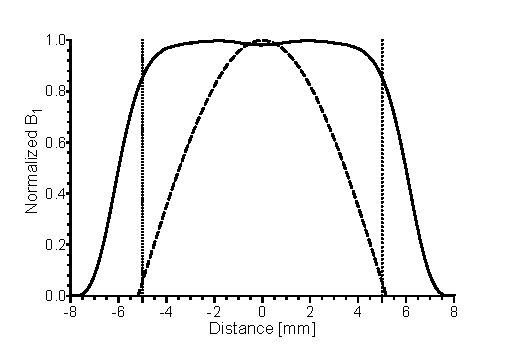
\includegraphics{Kapitel/Ch2-Images/02-TE01UProfile.eps}
 \caption[Ansys HFSS simulation of normalized B$_1$ field.]{Ansys HFSS simulation showing normalized B$_1$ field of the cylindrical re-entrant \cylTE{} (solid) compared to the cylindrical TE$_{\text{011}}$ cavity. Dotted lines mark the region-of-interest of the cylindrical re-entrant \cylTE{} cavity. }
 \label{Ch2-fig:normb1}
\end{figure}

If one designs a UF cylindrical \cylTE{} cavity with a region-of-interest of 10~mm, as described in Refs.~[3.\kern-0.4em\citenum{mett2001axially}] and [3.\kern-0.4em\citenum{anderson2002}], the B$_1$ variation over the cavity volume is reduced to 20\%. However, the overall $\Lambda_{max}$ is reduced by 39\% compared to a TE$_{011}$ cavity, due to the decrease in stored energy in the entire cavity volume. A solution to increase the resonator efficiency is to introduce re-entrant fins, shown in Fig.~\ref{Ch2-fig:GEO}B, where the electric field is concentrated, shown in \ref{Ch2-fig:EMFields}A, and results in a $\Lambda_{max}$ decrease of 11\% but an overall $\Lambda_{ave}$ increase of 59.6\%. The calculated resonator characteristics of the proposed UF re-entrant \cylTE{} cavity and comparison to a TE$_{011}$ and UF cylindrical \cylTE{} cavity are found in Table~\ref{Ch2-table:ansyschar}.

\begin{table}[htp]
\centering
\caption{Ansys HFSS simulated resonator characteristics.}
\label{Ch2-table:ansyschar}
\begin{tabular}{l|c|c|c}
Geometry & \begin{tabular}[c]{@{}l@{}}Cyl. TE$_{\text{011}}$ \\ D/L=1\end{tabular} & \begin{tabular}[c]{@{}l@{}}UF Cyl.\\ \cylTE{}\end{tabular} & \begin{tabular}[c]{@{}l@{}}UF \cylTE{}\\ Re-Entrant\end{tabular} \\ \hline \hline
Frequency & 34.3 & 34.5 & 34.1 \\ \hline
Q$_0$-Value & 13000 & 5900 & 1880 \\ \hline
Signal, S$_u$ & 1 & 0.73 & 1.06 \\ \hline
Signal, S$_s$ & 1 & 0.83 & 1.18 \\ \hline
$\Lambda_{max}$ {[}mT/W$^{1/2}${]} & 1.06 & 0.65 & 0.94 \\ \hline
$\Lambda_{ave}$ {[}mT/W$^{1/2}${]} & 0.52 & 0.52 & 0.83 \\ \hline
$\Delta$B$_1$ & 50.9\% & 20\% & 11.7\%
\end{tabular}
\end{table}

\begin{figure}[htp]\centering
 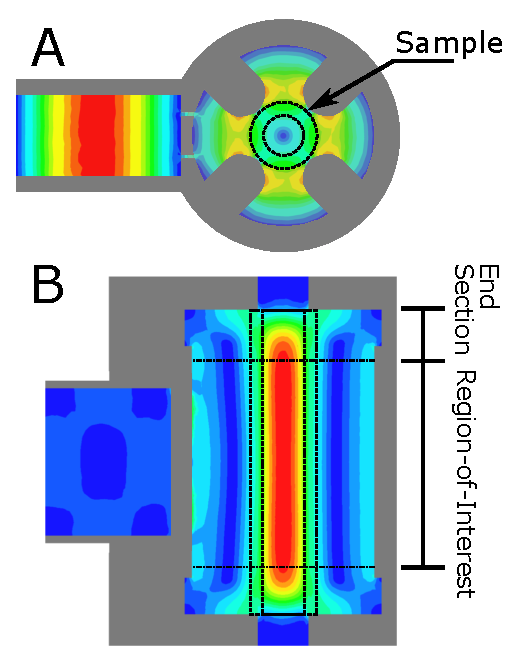
\includegraphics{Kapitel/Ch2-Images/03-TE01UEMFields.eps}
 \caption[Simulation of the microwave fields.]{Ansys HFSS simulation showing the magnitude of the microwave A) electric and B) magnetic fields of the uniform field re-entrant cylindrical \cylTE{} cavity. Each iris is 0.2~mm wide and extends over the entire waveguide length.}
 \label{Ch2-fig:EMFields}
\end{figure}

Using Ansys HFSS, a UF re-entrant \cylTE{} cavity is designed by the following procedure: (i) An eigen-mode solution of the central section with sample is simulated with a perfect magnetic field boundary condition. This provides the resonant frequency of the central section at cut-off with sample. (ii) The region-of-interest is extended to 10~mm and Rexolite end sections are added to the simulation at a nominal height. (iii) The end sections are varied until the eigen-frequency matches the cut-off frequency. (iv) An iris is introduced and the end sections are adjusted to accommodate the frequency shift. (v) Once completed, the resonator is imported into AutoDesk Inventor and prepared for fabrication. 

By properly matching the end sections, a uniform B$_1$ field can be realized, illustrated in Fig.~\ref{Ch2-fig:EMFields}B. The normalized B$_1$ field profile is shown in Fig.~\ref{Ch2-fig:normb1} as a solid line. In the 10~mm region-of-interest the B$_1$ field profile is 98\% uniform over the region-of-interest. 

As shown in Fig.~\ref{Ch2-fig:GEO}C, the re-entrant fins do not extend fully into the end section region. This design choice causes the end section to be electrically larger (shorter wavelength, $\lambda_g$) and reduces the end-section size needed to produce the matching criteria for the region-of-interest. Since the end sections are electrically larger, the roll-off is steeper compared to the re-entrant section. Decreasing the roll-off region of the resonator minimizes the sample volume that is excited by non-uniform fields.

\subsection{Dual-Slot Iris Design}

A dual-slot iris was designed in order to couple the UF re-entrant \cylTE{} cavity. The use of dual-slot irises reduce B$_1$ perturbations due to the stored energy in the iris. For UF resonators, the dual iris also reduces coupling to higher-order modes that may exist because of the large length of the region-of-interest. \cite{UFLGR2017} The size of a single capacitive iris needed to couple the resonator was 0.45~mm. A dual-slot iris with 0.2~mm thickness each was needed to achieve the same coupling. The geometry is shown in Fig.~\ref{Ch2-fig:GEO}A and C and the electric field profile in Fig.~\ref{Ch2-fig:EMFields}A.

\subsection{Waveguide H-type T-junction Coupler with Inductive Obstacles}
\begin{figure*}[htp]\centering
 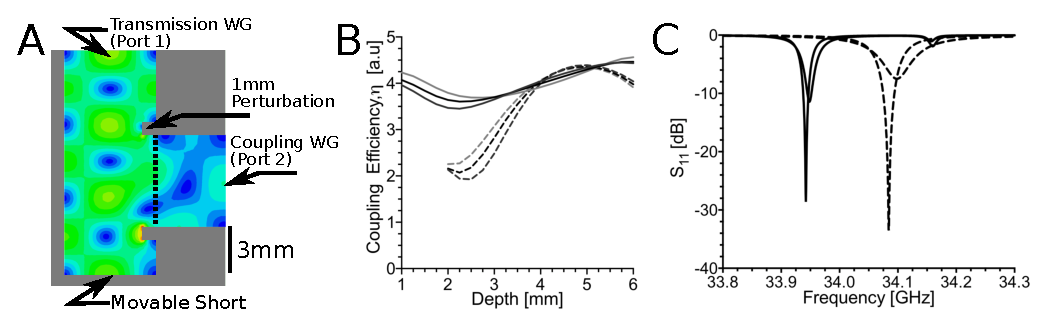
\includegraphics[width=\textwidth]{Kapitel/Ch2-Images/04-CouplingPert.eps}
 \caption[Waveguide H-type T-junction coupler geometry.]{A) Waveguide H-type T-junction coupler geometry with perturbations showing the transmission waveguide, coupling waveguide, and movable short. B) Ansys HFSS simulations showing the coupling efficiency without (solid) and with 1~mm perturbations (dashed) for three frequencies (33.5, 34, and 34.5~GHz, light grey, black, dark grey, respectively). C) Simulations showing the reflection coefficient S$_{\text{11}}$ without (solid) and with 1~mm perturbations (dashed) at various depths of the movable short (coupled and over-coupled; 3.5~mm and 5~mm). Operating frequency is 34.09~GHz.}
 \label{Ch2-fig:waveguide}
\end{figure*}

In order for the resonator assembly to fit in a 40~mm diameter cryostat, an H-type T-junction coupler was implemented with a sliding short matching system. This sliding short is typical for a Q-band TE$_{011}$ cavity and provides a robust coupling method for room temperature to sub-10~K measurements. \cite{generalte011} Typically coupling to a TE$_{011}$ cavity is performed by introducing an iris to the H-plane sidewall of the transmission waveguide. However, due to the oversized end-sections a coupling waveguide of 5.07~mm length is introduced perpendicular to the transmission waveguide, illustrated in Fig.~\ref{Ch2-fig:waveguide}A. 

Three features describe an H-Type T-junction coupler: (i) The H-type T-junction coupler is similar to the H-arm of a magic-Tee coupler. \cite{ramo1984fields, MITRadWaveguide} (ii) The coupling waveguide is at least $\lambda_g$/2 in length. (iii) In order to maximize coupling, an ``inductive obstacle'' on the sub-wavelength H-type T-junction is introduced to the transmission waveguide. The ``inductive obstacle'', described by Ref~[3.\kern-0.4em\citenum{MITRadWaveguide}] as a ``Window Formed by One Obstacle'', is introduced to the H-plane around the coupling waveguide and extend 1~mm into the transmission waveguide, illustrated in Fig.~\ref{Ch2-fig:waveguide}A. This inductive obstacle creates a favorable geometry for electric field coupling and increases the coupling efficiency. 

Plotted in Fig.~\ref{Ch2-fig:waveguide}B is the simulated coupling efficiency transmission can be calculated using an overlap integral \cite{born} of the two electric fields and is defined as
\begin{equation}
    \eta = \frac{\left| \int E_{t} \cdot E^*_{c} dA\right|^2}{\int \left|E_t\right|^2 dA \int \left|E_c\right|^2 dA},
\end{equation}
where $E_{t} \cdot E^*_{c}$ represents the electric field coupling over the waveguide interface area between the electric field of the transmission waveguide ($E_{t}$) and the coupling waveguide ($E_{c}$) at the interface area A, shown as a dotted line in Fig.~\ref{Ch2-fig:waveguide}A. 

The coupling efficiency between port 1 at the transmission waveguide and port 2 at the coupling waveguide is shown in Fig.~\ref{Ch2-fig:waveguide}B, where the coupling efficiency without the waveguide perturbations (solid) and with 1~mm perturbations (dashed) is plotted. Three frequencies (33.5, 34, and 34.5~GHz, light grey, black, dark grey, respectively) are used to show the frequency dependence. Lower coupling efficiency under-couples the resonator. The resonator is critically coupled when the movable short is around 3.5~mm depth at 34~GHz and maximum over-coupling occurs at 5~mm. The waveguide H-type T-junction coupler with the perturbation illustrates a more dynamic range in coupling for the same distance and a flatter response for maximum over-coupling with a 1~GHz frequency range. In order to produce the same coupling range without the waveguide perturbations the iris must be 25\% larger. A larger iris leads to inhomogeneity of the B$_1$ field around the iris and in the region-of-interest. 

The UF re-entrant \cylTE{} cavity is designed to be over-coupled. Shown in Fig.~\ref{Ch2-fig:waveguide}C is the effect of the movable short on the reflection coefficient S$_{\text{11}}$ of the UF re-entrant \cylTE{} with a range of coupling positions (3.5 and 5~mm, coupled and over-coupled). The resonator microwave frequency shift with coupling is reduced form 14.4~MHz to 8.2~MHz using the H-type T-junction coupler with perturbations. Lower microwave frequency pulling occurs due to a reduction in the stored energy in the region of the coupler. 

Additionally, for the same resonator geometry there is 145~MHz shift in operating frequency from its eigen-frequency of 34.1~GHz due to the impedance of the coupler without the perturbations. The coupler without perturbations has more stored energy and more reactance, consistent with the understanding of coupling systems with frequency dependence. \cite{Mett2009} This causes a shift in the real part of the microwave frequency to compensate for the imaginary part of the assembly reactance and makes the assembly more frequency dependent. 

\section{Results}
The Q$_0$-value of the UF cavity was measured to be 1330 with a distilled water ice sample at a frequency of 33.95~GHz. Additionally, the frequency shift of the re-entrant \cylTE{} cavity as match was adjusted from critically coupled (-45~dB ) to over-coupled (-9~dB) was 6.96~MHz shift. Consistent with simulations, see Fig.~\ref{Ch2-fig:waveguide}C. 

\begin{figure}[htp]\centering
 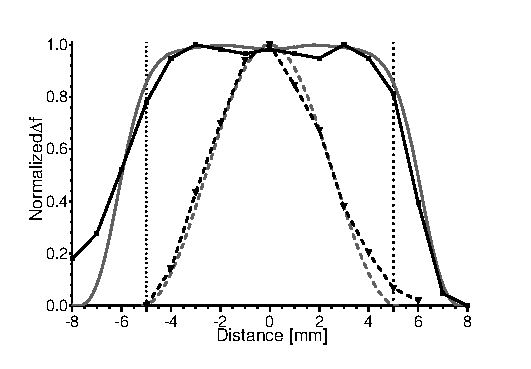
\includegraphics{Kapitel/Ch2-Images/05-TE01Uperturb.eps}
 \caption[Measured magnetic field using perturbing spheres.]{Method of perturbing spheres showing the normalized $\Delta$f along the axis of the cylindrical re-entrant \cylTE{} (solid) compared to the cylindrical TE$_{\text{011}}$ cavity. Dotted lines mark the region-of-interest of the cylindrical re-entrant \cylTE{} cavity.  Comparison to Ansys HFSS simulations are shown in grey.}
 \label{Ch2-fig:perturb}
\end{figure}

The change in frequency due to the presence of a small metallic probe is shown in Fig.~\ref{Ch2-fig:perturb}. Measurements of the UF re-entrant \cylTE{} cavity are shown as a solid line and a cylindrical TE$_{011}$ are shown as a dashed line. The profiles here should be compared to the Ansys HFSS simulations of Fig.~\ref{Ch2-fig:normb1}, repeated as gray for convenience. 

\begin{figure}[htp]\centering
 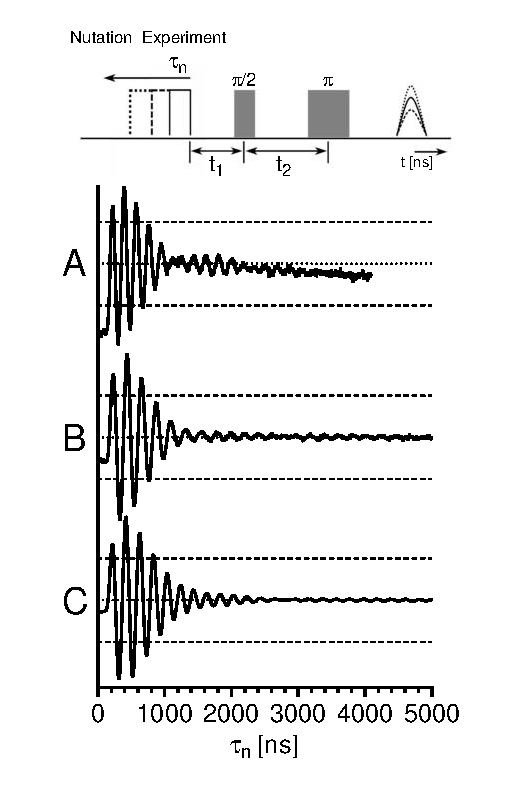
\includegraphics{Kapitel/Ch2-Images/06-Nutation.eps}
 \caption[Nutation experiment comparison.]{Nutation experiment on a BDPA sample performed using the A) cylindrical TE$_{011}$ cavity B) and the uniform field re-entrant \cylTE{} cavity with the sample extending the entire length and C) a 9.5~mm sample centered in the region-of-interest. Pulse lengths were 120~ns for $\pi$-pulse and the preparation pulse length was stepped 4~ns. Dotted lines show the nutation center, while dashed lines show 50\% signal markers.}
 \label{Ch2-fig:nutation}
\end{figure}

Shown in Fig.~\ref{Ch2-fig:nutation} are the data from the nutation experiment. Dotted lines represent the center of the nutations, while dashed lines show 50\% signal markers. The cylindrical TE$_{011}$ cavity data was taken with the BDPA sample extending the entire cavity length and plotted in Fig.~\ref{Ch2-fig:nutation}A. For a 120~ns $\pi$-pulse the power was set to 2.5~W. In Fig.~\ref{Ch2-fig:nutation}B, the UF re-entrant \cylTE{} cavity with the BDPA sample extending the entire cavity length is shown. For a 120~ns $\pi$-pulse the power was set to 5~W. A second sample with 9.5~mm length was centered in the UF re-entrant \cylTE{} cavity region-of-interest. Experimental nutation data are plotted in Fig.~\ref{Ch2-fig:nutation}C and for a 120~ns $\pi$-pulse the power was set to 5~W.

Nutation experiments show good results in terms of increased sensitivity and uniformity of the B$_1$ field. The nutations using the UF re-entrant \cylTE{} cavity with the sample extending the entire length show clear improvements over the data from the cylindrical TE$_{011}$ cavity, shown in Fig.~\ref{Ch2-fig:nutation}A and \ref{Ch2-fig:nutation}B, respectively. 

The UF re-entrant \cylTE{} cavity with the 9.5~mm sample only in the region-of-interest, shown in Fig.~\ref{Ch2-fig:nutation}C, has the nutations further extended and the initial off-set is further minimized. The Bruker E580 was only able to acquire 1000~ns of data, but with the 9.5~mm sample there was signal seen as far as 1300~ns. Increasing the integration would give even better signal. These data shows the advantages of uniform field cavities. Three differences of note are: (i) The nutations are improved by at least 40\% and the initial off-set is reduced by 50\%. (ii) The first-order linear background subtraction is not adequate for the cylindrical TE$_{011}$ cavity. Higher-order background exists that cannot be easily corrected. (iii) A nutation signal phase-inversion is exhibited in  Fig.~\ref{Ch2-fig:nutation}A at 1200~ns and another at 2400~ns, while only one inversion at 2800~ns is noticeable in Fig.~\ref{Ch2-fig:nutation}B. We have experimentally attributed this oscillatory phase-inversion to be due to inhomogeneity of the B$_1$ field, seemingly at the top and bottom of the resonator. The nutation signal phase-inversion is shown to be minimized in Fig.~\ref{Ch2-fig:nutation}C, but can be increased by moving the sample outside of the region-of-interest.

\section{Discussion}

Dielectric loading variations due to different samples change the cut-off frequency of the region-of-interest, and thus, the uniformity condition of the resonator. Shown in Fig.~\ref{Ch2-fig:dielectric} is the simulated microwave magnetic field squared (B$^2_1$) profile of the UF re-entrant cylindrical \cylTE{} cavity for a range of dielectric constants ($\epsilon_r$ ranges from 1 to 5 in integer steps, with a loss tangent of 0.005) for a fixed Rexolite end section geometry. The B$^2_1$ is used to highlight the differences and is proportional to EPR signal intensity. The frequency shift due to the real part of the dielectric from 1 to 5 is 34.492, 34.206, 33.910, 33.592, 33.264~GHz, respectively. 

\begin{figure}[htp]\centering
 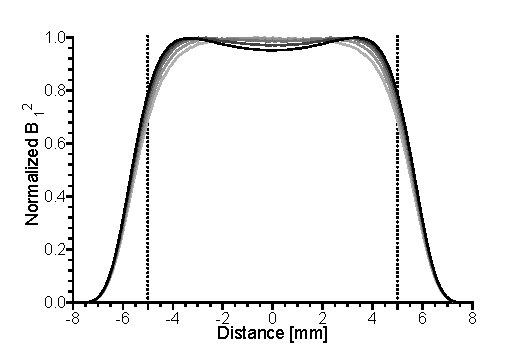
\includegraphics{Kapitel/Ch2-Images/07-TE01Udielectirc.eps}
 \caption[Ansys HFSS simulations of with varying samples.]{Ansys HFSS simulations of the microwave magnetic field squared (B$^2_1$) profile of the UF re-entrant cylindrical \cylTE{} cavity for a range dielectrics. The dielectric constant, $\epsilon$, is varied from 1 to 5 (dark to light) with a fixed end section geometry. Dotted lines mark the region-of-interest of the cylindrical re-entrant \cylTE{} cavity.  The B$^2_1$ is used to highlight the differences and is proportional to EPR signal intensity. }
 \label{Ch2-fig:dielectric}
\end{figure}

Although the resonator is designed for an $\epsilon_r$ of 3, good uniformity is exhibited for this limited range. This is an advantage of the UF re-entrant cavity compared to a UF cavity. Similar to a UF LGR, the electric field profile is more confined outside of the sample region and the B$_1$ field is stabilized by the current on the re-entrant fins. The B$_1$ uniformity over the entire sample volume varies from 80.1\%, 80.1\%, 79.8\%, 79.3\%, and	78.5\%, as the dielectric is stepped from $\epsilon_r$ 1 to 5, respectively.

The $\Lambda_{ave}$ of the UF re-entrant \cylTE{} resonator is lower than expected by about 40\%. This is mostly due to the Q$_0$-value being lower than expected. The lowering of the Q$_0$-value is due to the construction of the prototype resonator out of brass and higher losses in the Rexolite plastic than anticipated. Changing the resonator body to solid silver and experimenting with different plastics would be advantageous. 

Higher stored energy in the coupling and iris region makes the system more frequency dependent. The frequency dependence of the H-type T-junction coupler without inductive perturbations was shown to have a large effect on the coupling efficiency, shown in Fig.~\ref{Ch2-fig:waveguide}. Additionally, by extending the iris over the entire length of the waveguide H-plane, a long-slot iris is created. \cite{Mett2009} The long-slot iris exhibits lower stored energy than a resonant iris or inductive hole and minimizes B$_1$ field perturbations. By splitting the long-slot iris to a dual-slot iris, the stored energy and frequency dependence is further reduced. In general, the reduction of stored energy outside of the resonator reduces the frequency dependence when tuning, matching, or changing samples. These design criteria are critical for UF resonators. 

\begin{figure}[htp]\centering
 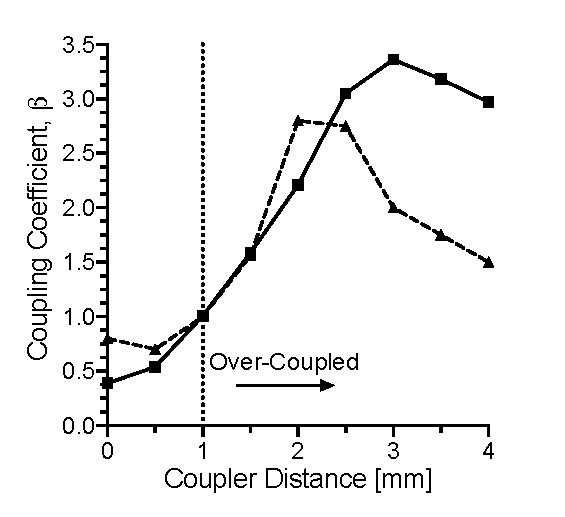
\includegraphics{Kapitel/Ch2-Images/08-couplingcoeff.eps}
 \caption[Bench measurements of the coupling coefficient.]{Bench measurements on the vector network analyzer of the coupling coefficient $\beta$  for the re-entrant \cylTE{} cavity with H-type T-junction coupler and long slot iris (solid) compared to the cylindrical TE$_{011}$ cavity with slot iris from Ref.~[3.\kern-0.4em\citenum{generalte011}] (dashed).}
 \label{Ch2-fig:coupling}
\end{figure}

Shown in Fig.~\ref{Ch2-fig:coupling} are vector network analyzer measurements of the coupling coefficient $\beta$ for the re-entrant \cylTE{} cavity with H-type T-junction coupler and long slot iris (solid) compared to the cylindrical TE$_{011}$ cavity with slot iris from Ref.~[3.\kern-0.4em\citenum{generalte011}]. The measured data shows better over-coupling performance for the re-entrant \cylTE{} cavity which corresponds to a larger bandwidth by the equation
\begin{equation}
    Q_L = \frac{Q_0}{\beta+1},
\end{equation}
where the loaded Q-value, Q$_L$, is proportional to bandwidth by $1/\Delta f$. \cite{ramo1984fields} With a lower initial Q$_0$ value, the re-entrant \cylTE{} cavity has a significant increase in bandwidth for comparable EPR signal. The re-entrant \cylTE{} cavity has a calculated bandwidth of approximately 110~MHz, while the cylindrical TE$_{011}$ cavity of Ref.~[3.\kern-0.4em\citenum{generalte011} has a calculated bandwidth of 46~MHz (Q$_0$ of 2400).

Finally, in the $x$- and $y$-direction the B$_1$ field exhibits some variation. A smaller inner diameter capillary (with the same outer diameter) could be used to improve this variation but will sacrifice EPR signal intensity. However, the $x$- and $y$-direction variation is already 15\% better in a re-entrant geometry compared to the cylindrical TE$_{011}$ cavity from both a ``sucking-in'' effect of the quartz capillary and more confined electric field profile, as shown in Fig.~\ref{Ch2-fig:EMFields}. The capillary geometry of 2.8~mm OD and 1.8~mm ID was chosen to be compatible with our current standard Q-band capillary tubes. 

\section{Conclusion}

A uniform field re-entrant cylindrical \cylTE{} cavity has been designed, fabricated, and tested to improve pulse EPR experiments. The microwave magnetic field, B$_1$, has been calculated and confirmed by measurements to be 88.3\% uniform over the entire cavity and 98\% uniform over the region-of-interest. By introducing re-entrant fins to a UF cylindrical \cylTE{} cavity, the Q-value of the re-entrant \cylTE{} cavity is lowered, but the resonator efficiency and stored energy is increased. This new geometry yields similar signals as the standard cylindrical TE$_{011}$ while increasing $\Lambda_{ave}$ by approximately 60\%. The increase of $\Lambda_{ave}$ affects pulse EPR experiments in two ways: (i) less microwave power is needed for the same tip angle; and (ii) the majority of the sample is excited at the same tip angle. 

Initial results using a brass prototype resonator have shown significantly improved data quantified by the nutation experiments. In this work, we have shown that a UF re-entrant geometry can provide an enhanced efficiency parameter, increase EPR signal intensity, larger bandwidth and a uniform microwave magnetic field along the sample volume to improve pulse EPR experiments. Future work includes a second generation resonator in solid silver, ESEEM, HYSCORE and ELDOR-detected NMR experiments (EDNMR), and extending the UF re-entrant \cylTE{} cavity to W-band frequencies.

{\renewcommand{\bibsection}{\clearpage\section*{\bibname}\markboth{\bibname}{\bibname}}
\renewcommand{\bibname}{CHAPTER 3. REFERENCES}
\bibliographystyle{elsarticle-num}
\bibliography{Kapitel/Ch3-References}   % name your BibTeX data base
}